\documentclass[10pt,a4paper]{article}
\usepackage[T1]{fontenc}
\usepackage[scaled]{helvet}
\usepackage{cite}
\usepackage{url}
\usepackage{graphicx}
\usepackage{listings}
\usepackage{float}
\usepackage{amsmath}
\usepackage{amssymb}
\usepackage{fancyhdr}
\usepackage{lastpage}
\floatstyle{boxed} 
\restylefloat{figure}
\renewcommand*\familydefault{\sfdefault}
\title{Threads and CPU Scheduling}
\author{David Lynch - david.lynch@raglansoftware.com }
\begin{document}
\maketitle
\begin{abstract}
In this article we will look at common algorithms that CPU schedulers will implement. You'll find that these algorithms are relevant to other areas in which queues exist and decisions are made, so a clear understanding of the theory and implementation of these is essential. Thereafter, we will talk about threads, which are a very important means for a process to execute concurrently without explicitly forking. 
\end{abstract}
\section{Threads}
Up to now we have considered process as an entity that will execute a single program in a {\bf single thread of control}. This means that internally, the process will execute only one code path concurrently. Separately, these single threaded processes will run concurrently with other processes. However, there are major advantages of facilitating concurrency within a process. A {\bf multi-threaded} application can run several code paths concurrently within a process. The advantage of being within the process is that there is seamless sharing of code, external resources such as files and a shared memory area. Coupled with this each thread will have a private stack area and an entry in the process control block that allows the saving of state and registers that are only associated with the thread itself. This illustrated in figure \cite{processthread}. Further advantages include allowing applications to execute something else while blocked. For example, show a loading spinner while waiting for an image to download in the background. Economically, the cost of a context switch between threads is much less than that of a context switch between processes. Since the text section of the process, as well as shared resources and memory, do not all need to be saved or re-initialized after a switch, there is a lot less work to do. 
\begin{figure}
\caption{A multi-threaded process. \cite{OSCONCEPTS}}
\begin{center}
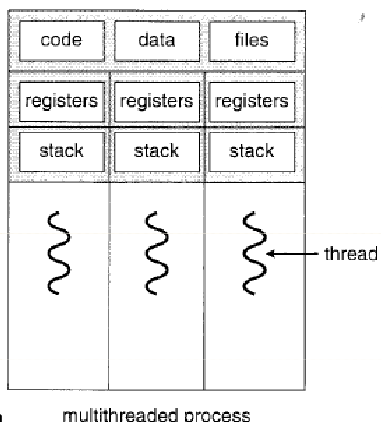
\includegraphics[scale=0.45]{../images/multi-threaded-process.png}
\label{processthread}
\end{center}
\end{figure}
\subsection{Multi-Threading Models}
The operating system will facilitate user programs via {\bf user threads} and will also facilitate concurrency in kernel space by supporting and managing {\bf kernel threads}. There must exist some mapping between the user threads and the kernel threads.
\subsubsection{Many-to-One}
In this scenario many threads are mapped to one kernel thread. This makes it particularly easy to manage threads at the application layer. The cost of switching between threads in the application layer is reduced further, since the switch is a soft one. The downside of this approach is that if two of the user threads make a blocking kernel thread call, we end up with blocking across the whole application. GNU portable threads are an example of a library that takes this approach.  
\subsubsection{One-to-One}
A more common approach is an explicit mapping between a user thread and a kernel thread. This allows multiple threads to execute in parallel on different processors, and allows a greater degree of concurrency at the application layer by not exposing these threads to blocks that are caused by the other application layers. If you think of a typical Windows Application a common use case is to display an animated message on the screen while a file is loading. In the previous case, the file I/O would block the single kernel thread and we could not show anything. In this case, we can execute concurrently. On a single processor system, the animated messages' processing is interleaved with the I/O wait quite efficiently. In the dual core approach they may be really executed in parallel to some degree. The downside to this approach is cost. Due to the common use case I just described, you will find that operating systems such as Windows and Linux take this approach. 
\subsubsection{Many-to-Many}
Some operating systems provide a hybrid approach whereby a pool of kernel threads is maintained, and the user threads are mapped on an as-needed basis. The idea here is to multiplex onto a smaller number of kernel threads in order to manage down somewhat the overhead exhibited by the one-to-one mapping. At the same time, this approach mitigates against inter thread blocking to some degree. This degree is configurable and related to the size of the kernel thread pool. As the thread pool increases in size, the cost of management of these threads increases. HP-UX is an operating system that will take this approach. This is typically deployed in server environments that have less requirements on responsiveness but greater requirements on throughput and CPU utilization. 
\subsection{Libraries}
There are a number of common libraries that provide an API for the creation and management of threads. Some of these libraries will exist only in user space, but are more typically supplemented by kernel level support. At the system level, these libraries can be quite complex. Some threading libraries, such as the Java language threading libraries, will attempt to abstract away the complexity of the system level libraries somewhat by wrapping a subset of its functionality and exposing it as another API. 
\subsubsection{POSIX pThreads}
PThreads \cite{pthreads} expose a user or kernel level library. 

ADD PTHREAD LISTING

\subsubsection{Win32 Threads}
Win32 Threads \cite{win32threads} are exposed at the kernel level 

ADD WIN32 THREAD LISTING

\subsubsection{Java Libraries}
Java Libraries \cite{javathreads} are implemented over whatever native libraries are in use on the host operating system. 

ADD JAVA LISTING
\newline\newline (FLESH THIS OUT)

\subsection{Thread Management}
There are a number of issues to consider when managing threads that are somewhat analogous to the management of processes. 
\subsubsection{Thread Creation}
A thread creation  must only happen by means of a fork that will {\it duplicate the creating thread only}. An execution of the {\bf exec} system call will not only duplicate the calling thread but the entire process, including any other threads that exist in the calling application. 
\subsubsection{Thread Cancellation}
A thread must either terminate itself, or be terminated by some other thread. When termination of a thread is requested it can be executed {\bf asynchronously} whereby the OS does not wait around for the thread to terminate gracefully. Alternatively, {\bf deferred cancellation} causes the operating system to periodically check if the thread is ready for termination, usually giving it warning and the opportunity to cancel itself. Graceful cancellation by the thread assists in the effective reclamation of resources, state and shared memory. In a forced termination, these are all executed immediately. If the thread to be executed has not {\bf checkpointed} it's state, that state will be lost giving in unpredictable results.  
\subsubsection{Signal Handling}
A signal, or event handler, is code that gets executed when the OS, program or user tries to communicate with the thread. The OS is responsible for the guarantee of delivery. There are synchronous signal handlers that require immediate action. Examples of such are illegal memory access, errors such as division by zero. Asynchronous signals do not require immediate handling, but there may be a time period after which an asynchronous signal will become a synchronous one. The most common example is the user action {\it ctrl+c} which forces a process to exit. A default signal handler will almost always be provided by the underlying library. We will only replace this handler if we require special behaviour to occur as the signal is handled.   
\subsubsection{Thread Pools}
As the number of threads increases, the cost of managing these threads also increases. This may not necessarily be a linear function. At some point the presence of huge amounts of threads on a system causes so much context switching that it would be better to execute in a single threaded fashion. Furthermore, there is a cost to creating a new thread. So much so that it may not be enough to simply create these threads on demand. For these two reasons thread pools are created by both the operating system and the user applications. They are typically initialized in bulk as an up-front cost and are set to a fixed, or semi-fixed size. These pools sit idle until they are given work. When the pool has been exhaused, either the request for a new thread fails due to lack of resources, or some space in the pool is freed up. When there is a free thread in the pool and a new thread is requested, a thread in  the pool is immediately assigned some work. This can have a positive effect on the response time of the request. Web Servers will sit around with thread pools that are waiting to handle requests for web pages from users. Since for every request we do not have to create new threads, the user experience is significnatly improved. Tuning thread pools in terms of size is often an empricial process. Designing your application to leverage thread pools is more of an architectural decision.
\subsubsection{Thread Specific Data}
Threads my need their own copies of data that may be duplicated in the shared memory space or may be totally scoped locally to the thread. This in particular allows partial results of work on threads to be stored before they are ready for sharing with other threads. The Java {\it ThreadLocal } class facilitates this behaviour. It provides an area for Threads to store standard variables, with the cavieat that each time a thread will store a particular value named by a key, a unique copy of the data is created that is exclusively accessable by the thread \cite{threadlocal}. A good use of this facility is in situations where you need to share state accross the thread, but the state is only relevant in the context of the thread.  
\section{CPU Scheduling}
\subsection{Pre-Emptive Scheduling}
\subsection{The Dispatcher}
\subsection{Scheduling Criteria}
\subsection{FCFS - First Come First Served}
\subsection{SJF - Shortest Job First}
\subsection{RRS - Round Robin Scheduling}
\subsection{Multi-Level Queue Scheduling}
\subsection{Multi-Processor Scheduling}
\subsection{Thread Scheduling}
\subsection{Scheduling Algorithm Evaluation}
\subsection{Windows XP}
\subsection{Linux}



\bibliography{../biblio/techfundamentals.bib}{}
\bibliographystyle{plain}
\begin{center}
{\small \copyright  David Lynch 2012. Do not reproduce without written permission.}
\end{center}
\end{document}
